\chapter{Teoría de la forma}\label{formahistorica}

\section{La teoría de la forma de Borsuk}

La primera vez que la palabra <<forma>> es usada en el sentido del que nos ocupamos en este trabajo se sitúa en la conferencia de Karul Borsuk \textit{Concerning the notion of the shape of compacta} en el International Symposium on Topology and its Applications, celebrado en Herzegovina en agosto de 1968 \cite{borsuk1969concerning}. No obstante, el contenido de esta conferencia había sido publicado previamente en el artículo fundacional \textit{Concerning homotopy properties of compacta} \cite{Borsuk_1968} de Borsuk.

Borsuk observó que muchos de los teoremas más importantes en la teoría de homotopía solo son válidos en espacios con buen comportamiento local, pero fallan en espacios como los compactos métricos. El autor buscaba ampliar esta teoría para que capturase mejor las propiedades topológicas globales de los espacios, con una idea similar a la que ya había expuesto D. E. Christie a\~nos antes en \textit{Net homotopy for compacta} \cite{christie1944net}: en vez de considerar aplicaciones de $ \mathbb{S}^n$ en el espacio, las consideró en entornos del espacio cada vez más peque\~nos, puesto que estos no tenían esas malas propiedades locales pero podían seguir capturando las globales. De esta forma, también se podían definir aplicaciones entre espacios como aplicaciones entre sus entornos para llegar a una nueva noción de homotopía, y a una nueva categoría. Christie ya observó que esta vía era equivalente a la propia teoría de homotopía en espacios con regulares localmente como los ANR's. 

Antes de describir la forma según Borsuk, hagamos un excurso para estudiar cómo esta idea informal es provechosa en el paradigmático y clásico ejemplo del \emph{Círculo de Varsovia}: 
\begin{figure}[h]
  \centering
  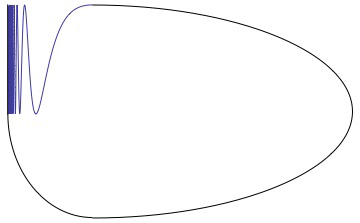
\includegraphics[scale = 0.8]{imagenes/Warsaw-circle.png}
  \caption{El círculo de Varsovia.}
  \label{circulovarsovia}
\end{figure}

Este espacio es conexo por caminos y simplemente conexo, de tal forma que la aplicación $ f:X\lra \{*\} $ induce isomorfismos en todos sus grupos de homotopía. Sin embargo, no se cumple en él el Teorema de Whitehead, puesto que no hay una equivalencia homotópica entre ambos: si la hubiera, pongamos $ H(x,0) = \id_{X} $ y $ H(x,1) = \{a\} $, entonces $ h_x(t) = H(x,t ) $ constituiría un camino uniendo $ x  $ y $ a  $. Por las propiedades del Círculo de Varsovia, sabemos que un tal camino no puede pasar por el tramo irregular, de tal forma que los puntos en la línea contigua a dicho tramo viajan a su imagen dando la vuelta por debajo y los puntos infinitamente próximos del tramo lo hacen superando las ondas, contra la continuidad de $ H  $. Sin embargo, las aplicaciones de $ \mathbb{S}^1 \lra U_n $ donde los $ U_n  $ son entornos de $ X  $ cada vez más cercanos sí se hacen cargo de su similitud con la circunferencia, y de hecho el grupo de dichos lazos es $ \Z  $, como lo es el grupo fundamental de la circunferencia.

Volvemos a la descripción de la forma de Borsuk. Borsuk considera espacios métricos compactos $ X, Y  $ inmersos en el cubo de Hilbert $ Q  $, y estudia sucesiones de aplicaciones entre sus entornos que llama \textbf{sucesiones fundamentales}, $ f_n:Q\lra Q  $ tales que
\begin{itemize}
  \item[] para todo entorno $ V$ de $Y  $ existe un entorno $ U  $ de $ X  $ (todos ellos en $ Q  $) que cumple $ f_n(U)\subc V  $ y $ \rest{f_n}{U} \simeq \rest{f_{n+1}  }{U }$ para casi todo $n$.
\end{itemize}
Dos sucesiones $ \underbar{f}, \underbar{g} $ son homótopas si todo entorno $ V  $ de $ Y  $ admite un entorno $ U  $ de $ X  $ tal que $ \rest{f_n}{U}\simeq \rest{g_n}{U} $ para casi todo $ n $. Esto define una relación de equivalencia entre sucesiones  que las divide en \textbf{clases fundamentales}. Podemos comprobar que la composición de clases componiendo sus representantes es una operación bien definida \cite[p. 232]{Borsuk_1968} y que la sucesión $ (\id_X ) $  es fundamental. Obtenemos así una categoría $ \Sh_B $ cuyos objetos son los compactos en $ Q $ y sus morfismos las clases fundamentales. Tal y como hacíamos en homotopía, diremos que dos espacios $ X$ e $Y $ tienen la misma \textbf{forma} si existen clases fundamentales $ [\underbar{f }]:X\lra Y  $, $ [\underbar{g}]:Y\lra X  $ tales que $ [\underbar{f}][\underbar{g}]  = [\id_{Y }] $ y $ [\underbar{g}][\underbar{f}]  = [\id_X ] $.     

Siguiendo a Christie, Borsuk presenta otro acercamiento a la forma a través de lo que denomina \textbf{aplicaciones aproximativas}: dados dos compactos $ X,Y\subc Q  $, son sucesiones de aplicaciones $ f_n: X\lra Q  $ tales que 
\begin{itemize}
  \item[] para todo $ V  $ entorno de $ Y  $ se tiene $ f_n\simeq f_{n+1}  $ en $V$ para casi todo $ n $.
\end{itemize}
Entre aplicaciones aproximativas también podemos definir una noción de homotopía, y diremos que $ (\vf_n) $ y $ (\psi_n) $ son homótopas si para todo entorno $ V  $ de $ Y  $ tenemos $ \vf_n\simeq \psi_n  $ en $ V  $ para casi todo $ n  $. De nuevo, esto define una relación de equivalencia a cuyas clases llamaremos \textbf{clases aproximativas}. Observamos que, aunque no podemos componer clases aproximativas porque los dominios no coinciden, sí podemos definir la composición de clases fundamentales con clases aproximativas componiendo representantes. Si asociáramos a cada clase aproximativa una fundamental, podríamos definir una categoría mediante esta operación. 

\begin{theorem}
  Existe tal asociaci'on y nos permite definir una categoría de compactos métricos que tiene por morfismos las clases aproximativas y es isomorfa a $ \Sh_B  $.
\end{theorem}
\begin{proof}
  Dada una aplicación aproximativa $ \vf = (\vf_n):X\lra Q  $, podemos extender cada aplicación $ \vf_n:X\lra Q  $ a una $ \Phi_n:Q\lra Q  $ porque el cubo de Hilbert es un AE. Todo entorno abierto $ V $ de $ Y  $ en $ Q  $ es abierto de un ANE, así que es ANE y, por tanto, ANR. Como $ \rest{\Phi_n}{X} \simeq \rest{\Phi_m}{X} $ en $ V  $, el Teorema \ref{extensionhomotopia} asegura que podemos extender esta homotopía de tal forma que $ (\Phi_n) $ sea una sucesión fundamental.

  Si tomamos otra aplicación aproximativa $ \psi = (\psi_n) $ homótopa a $ \vf  $, tenemos que las sucesiones fundamentales asociadas a cada una, $ \Psi  $ y $ \Phi  $ respectivamente, cumplen que para todo $ V $ entorno de $ Y  $ en $ Q  $,
  \begin{gather*}
    \rest{\Phi_n }{X } = \vf_n \simeq \psi_n  = \rest{\Psi_n }{X} \text{ en } V \text{ para casi todos } n,m .
  \end{gather*}
  De nuevo por el Teorema \ref{extensionhomotopia} podemos extender esta homotopía y, por tanto, la correspondencia establecida respeta las clases aproximativas. Esto significa que la composición de clases aproximativas $ [\psi]\circ [\vf ] $ está bien definida como $ [\Psi]\circ [ \vf ] $. Llamaremos a esta correspondencia $ F  $. Observamos que 
  \begin{gather*}
    F([\psi]\circ [\vf]) = F([\Psi \circ \vf])  \quad  \& \quad F([\psi])\circ F([\vf]) = [\Psi]\circ [\Phi ] = [\Psi \circ \Phi ]. 
  \end{gather*}
  Si tenemos un representante $ \Gamma  $ de $ F([\Psi \circ \vf]) $, es claro que para todo $ V  $ entorno de $ Y  $ en $ Q  $,
  \begin{gather*}
    \rest{\Gamma_n }{X} \simeq \Psi_n \circ \vf_n  = \rest{\Psi_n\circ \Phi _n}{X} \text{ en } V \text{ para casi todos } n,m,
  \end{gather*}
  de donde $ F  $ es un funtor por el argumento anterior. 

  La restricción a $ X  $ de una sucesíon fundamental $ \underbar{f} = (f_n):Q\lra Q  $ es una clase aproximativa por definición y, si dos sucesiones son homótopas, dichas clases lo son también. Además, la restricción conmuta con la composición y, por ende, esta asociación trivial es el funtor inverso de $ F  $. Esto implica que $ F  $ es un isomorfismo de categorías, como queríamos demostrar.
\end{proof}

Será útil más adelante tener en cuenta esta correspondencia entre aplicaciones aproximativas y sucesiones fundamentales. Mediante la noción de clase aproximativa se definen operaciones de producto e inversión y se da estructura de grupo a las clases aproximativas de $ \mathbb{S}^n\lra Y  $, lo que se llama el $ n $\textbf{-ésimo grupo de homotopía fundamental} de $ Y  $. De hecho, toda clase fundamental entre dos espacios induce de manera funtorial un homomorfismo entre sus grupos fundamentales\footnote{No confundir con el grupo fundamental de teoría de homotopía clásica.} y aunando ambas afirmaciones se obtiene un funtor $ \Sh_B \lra \text{Ab} $ para $ n>1  $ y en Grp para $ n=1 $.

Como afirmamos al principio, toda esta teoría se puede ver como una extensión interesada de la teoría de homotopía, puesto que sobre los espacios con buenas propiedades locales como los ANR's, coinciden. Esto es consecuencia de los siguientes hechos:
\begin{enumerate}
  \item Toda aplicación $ f:X\lra Y  $ se puede extender a una $ \hat{f}:Q\lra Q  $ por ser $ Q  $ un AE y $ X  $ cerrado en $ Q  $. Así, podemos formar una sucesión fundamental $ (f_n )_n  $ con $ f_n =  \hat{f} $.
  \item  \label{punto2} Si dos aplicaciones son débilmente homótopas, es decir, homótopas en cada entorno $ V  $ de $ Y  $ en $ Q  $, sus sucesiones fundamentales inducidas son homótopas. 
  \item La clase fundamental $ [\hat{f}] $ no depende de la extensión escogida.
  \item Si $ Y  $ es un ANR, toda clase fundamental $ [\underbar{f}]:X\lra Y  $ viene inducida por una aplicación $ f:X\lra Y  $.
  \item Si dos aplicaciones $ f,g:X\lra Y  $ generan la misma clase fundamental, entonces son débilmente homótopas.\label{punto5}
  \item Si dos aplicaciones entre ANR's son débilmente homotópas, entonces son homótopas. \label{punto6}
  \item Si dos ANR $ X  $ e $ Y  $ tienen la misma forma, entonces tienen el mismo tipo de homotopía. \label{punto7}
  \begin{proof}[Demostraci'on del Punto \ref{punto7}]
    Sean $ [\underbar{f}] $ y $ [\underbar{g}] $ las clases que nos dan la equivalencia de forma. Por ser ambos espacios ANR's, ambos morfismos vienen inducidos por aplicaciones continuas $ f:X\lra Y  $, $ g:Y\lra X  $. Como $ [g][f] = [\id_X ] $ y $ [f][g] = [\id_Y] $, son débilmente homótopas por el punto \ref{punto5}, y por el punto \ref{punto6} son homótopas.
  \end{proof}
\end{enumerate}
Como corolario de este desarrollo también podemos deducir que si dos espacios tienen el mismo tipo de homotopía, la equivalencia homotópica induce una equivalencia fundamental por el punto \ref{punto2} y tienen la misma forma. 

Después de la publicación del artículo de Borsuk, diversos autores intentaron generalizar la teoría más allá de los compactos métricos mediante nuevas aproximaciones. En 1970, S. Marde\v si\'c y J. Segal definieron la forma en espacios Hausdorff compactos \cite{Mardešić1970,Mardešić1971}, iniciando el acercamiento por sistemas inversos a la forma y poniendo la base para la generalización categórica del concepto, que vendría de la mano de Morita para espacios topológicos en general \cite{Morita1975}. Mientras tanto, Fox \cite{Fox1972} y  Borsuk \cite{borsuk1975} la generalizarían por distintas vías a espacios métricos generales. En Espa\~na, J. M. Sanjurjo dio una nueva descripción de la categoría forma basada en las aplicaciones multivaluadas \cite{sanjurjo_1990,sanjurjo_1992} que más tarde revisarían M. A. Morón y A. González \cite{ALONSOMORON2008972}.

Más progresos de la teoría siguieron llegando, consiguiendo probar teoremas análogos a los de Whitehead, Hurewicz \cite{Morita1975} y Smale \cite{dydak1978whitehead} sin las condiciones locales que aparecían como necesarias en la teoría de homotopía. Otra fuente de aplicaciones de la teoría de la forma serían los sorprendentes teoremas sobre complementos demostrados por Chapman \cite{chapman1972some,chapman1972shapes}, quien consiguió caracterizar la forma de un compacto métrico mediante el tipo topológico de su complementario en $ Q  $. 




\section{La forma mediante ANR-sistemas}\label{seccionanr}
En esta sección vamos a generalizar la teoría de la forma a compactos Hausdorff basándonos en el artículo \textit{Shape of compacta and ANR-systems} de S. Mard\v esi\'c y J. Segal \cite{Mardešić1971}. Esta descripción fue rápidamente generalizada a un nivel más abstracto que visitaremos en el Cap'itulo \ref{formacategorica}. La filosofía consistirá en asociar a cada espacio un sistema de espacios ANR y estudiar los morfismos entre estos sistemas, emulando lo que hacíamos mediante los entornos y las sucesiones fundamentales.

En lo que sigue, cuando hablemos de un ANR nos referiremos a un compacto ANR para la categoría de espacios métricos; cuando hablemos de un espacio $ X  $, será de la categoría Cpt de espacios compactos Hausdorff. 

\begin{definition}
    Diremos que un conjunto parcialmente ordenado $\Lambda $ es \textbf{dirigido} si, para todos $\lam_1,\lam_2\in \Lambda $, existe un $\lam\in \Lambda $ mayor que ambos, $\lam_1,\lam_2\leq \lam $. Diremos que es \textbf{cofinito} si el conjunto de predecesores de todo 'indice es finito. Un subconjunto $\Lambda'\subc \Lambda $ es \textbf{cofinal} si, para todo $\lam\in \Lambda $, existe $\lam'\in \Lambda ' $ tal que $\lam\leq \lam'$.
\end{definition}


\begin{definition}
  Sea $ \ccal  $ una categoría. Un \textbf{sistema inverso} $ \mathbf{X } $ en $ \ccal  $ está formado por un conjunto dirigido de índices $ \Lambda  $, un objeto $ X_\lambda  $ para cada $ \lambda \in \Lambda  $ y un \textbf{morfismo de paso} $ p_{\lam \lam' } : X_{\lam'} \lra X_\lam $ para cada par $ \lam\leq \lam'  $. Estos morfismos han de cumplir $ p_{\lam \lam }  = \id_{X_\lam } $ y que si tenemos $ \lam\leq \lam' \leq \lam''  $ entonces $ p_{\lam \lam'}p_{\lam'\lam ''} = p_{\lam \lam' } $. Si $ \Lambda  = \N  $, diremos que $ \mathbf{X } $ es una sucesión inversa.
\end{definition}

Diremos que un sistema inverso es un \textbf{ANR-sistema}\footnote{La traducci'on cl'asica al espa\~nol de este concepto es <<sistema de ANR's>>. En este texto preferimos <<ANR-sistema>> porque acorta la escritura y es m'as conveniente.} si el conjunto dirigido es cofinito, cada $ X_\lam  $ es un ANR y los morfismos de paso son funciones continuas. Dado un ANR $ X  $, podemos construir un ANR-sistema trivial asociado haciendo $ X_\lam = X  $ y $ p_{\lambda\lambda'} = \id_X  $. Un \textbf{morfismo de ANR-sistemas} o \textbf{ANR-morfismo} $ \mathbf{f}:\mathbf{X} = (X_\lam,p_{\lam\lam'},\Lambda)\lra \mathbf{Y} = (Y_\mu,q_{\mu\mu'},M )  $ consiste en una función creciente $ \vf:M \lra \Lambda  $ y aplicaciones $ f_\mu :X_{\vf(\mu)}\lra Y_\mu  $ tales que para todo $ \mu $, si $ \mu\leq \mu'  $, el siguiente diagrama conmuta en homotopía\footnote{A partir de aquí, cada vez que nos refiramos a la conmutatividad de un diagrama, será en homotopía a no ser que se especifique lo contrario.}:
\begin{center}
  \begin{tikzcd}
    X_{\vf(\mu)}\arrow{d}{f_\mu} & X_{\vf(\mu')} \arrow{d}{f_{\mu'}}\arrow{l} \\ 
    Y_\mu & Y_{\mu'} \arrow{l}
  \end{tikzcd}.
\end{center}
 Si cambiamos los sistemas por Cpt-sistemas, obtenemos un \textbf{Cpt-morfismo}. Denotaremos los morfismos desde un sistema trivial $(X,\id_X) $ como $\mathbf{f}:X\lra \mathbf{Y}$. El morfismo identidad es $ \mathbf{\id_\mathbf{X}} = (\id_{X_\lam},\id_\Lambda) $. La composición de dos morfismos $ (f_\mu, \vf ) $ y $ (g_\alf, \psi ) $ se define como el morfismo $ (g_\alf\circ f_{\psi(\alf )}, \vf\circ \psi ) $, y está bien definida por la conmutatividad de
\begin{center}
  \begin{tikzcd}
    X_{\vf\psi(\alf')} \arrow{d} \arrow{r}{f_{\psi(\alf')}} & Y_{\psi(\alf')} \arrow{r}{g_{\alf'}} \arrow{d} & Z_{\alf'} \arrow{d} \\ 
    X_{\vf\psi(\alf)} \arrow{r}{f_{\psi(\alf)}} & Y_{\psi(\alf)} \arrow{r}{g_{\alf}} & Z_\alf 
  \end{tikzcd}.
\end{center}

Diremos que dos morfismos de ANR-sistemas $ \mathbf{f},\mathbf{g}:\mathbf{X}\lra \mathbf{Y} $ son homótopos, $ \mathbf{f}\simeq \mathbf{g} $, si para todo $ \mu\in M  $ existe un índice $ \lam\geq \vf(\mu),\psi(\mu ) $ tal que el siguiente  diagrama conmuta:
\begin{center}
  \begin{tikzcd}
    X_{\vf(\mu)}\arrow[swap]{dr}{f_\mu} & X_{\lambda} \arrow[r] \arrow[l] & X_{\psi(\mu)} \arrow{dl}{g_\mu} \\ & Y_\mu &
  \end{tikzcd}.
\end{center}
Es rutinario comprobar que esta relación es de equivalencia por la conmutatividad del diagrama 
\begin{center}
  \begin{tikzcd}
    & & X_{\lam''}\arrow{dr}\arrow{dl} & & \\ 
    X_{\vf(\mu)} \arrow{drr}{f_\mu} & X_\lam \arrow{r}\arrow{l} & X_{\psi(\mu)} \arrow{d}{g_\mu} & X_{\lam'}\arrow{r} \arrow{l} & X_{\chi(\mu)} \arrow{dll}{h_\mu}\\ 
    & &Y_\mu & & 
  \end{tikzcd}
\end{center}
tomando $ \lam'' \geq \lam,\lam'  $. De hecho, esta relación de equivalencia respeta la composición de morfismos: si tenemos $ \mathbf{f},\mathbf{f}':\mathbf{X}\lra \mathbf{Y} $ y $ \mathbf{g},\mathbf{g}':\mathbf{Y}\lra \mathbf{Z } $ homótopos dos a dos, 
\begin{enumerate}
  \item primero, probamos que $ \mathbf{g}\mathbf{f}\simeq \mathbf{g}'\mathbf{f} $: existe un $ \mu\geq \psi(\alf),\psi'(\alf) $ tal que el siguiente diagrama conmuta:
  \begin{center}
    \begin{tikzcd}
      X_{\vf\psi(\alf)} \arrow{d}{f_{\psi(\alf)}} & X_{\vf(\mu )} \arrow{r} \arrow{d}{f_\mu} \arrow{l} & X_{\vf\psi'(\alf)} \arrow{d}{f_{\psi'(\alf)}} \\ 
      Y_{\psi(\alf)} \arrow{dr}{g_\alf} & Y_\mu \arrow{r} \arrow{l}  & Y_{\psi'(\alf)} \arrow{dl}{g_\alf} \\ 
      & Z_\alf &
    \end{tikzcd};
  \end{center}
  \item segundo, observamos que $ \mathbf{g}\mathbf{f}\simeq \mathbf{g}\mathbf{f}'  $ porque existe $ \lam\geq \vf\psi(\alf),\vf'\psi(\alf) $ que hace conmutativo
  \begin{center}
    \begin{tikzcd}
      X_{\vf\psi(\alf)} \arrow{dr}{f_{\psi(\alf)}} & X_\lam \arrow{r} \arrow{l} & X_{\vf'\psi(\alf)} \arrow{dl}{f_{\psi(\alf)}} \\ & Y_{\psi(\alf)} \arrow{d}{g_\alf} & \\ & Z_\alf & 
    \end{tikzcd}
  \end{center}.
\end{enumerate}
Diremos que un ANR-morfismo $ \mathbf{f} $ es una \textbf{equivalencia homotópica} si existe $ \mathbf{g} $ tal que $ \mathbf{g}\mathbf{f}\simeq \id_X  $ y $ \mathbf{f}\mathbf{g}\simeq \id_Y  $. Diremos que dos sistemas tienen el mismo \textbf{tipo de homotopía} si existe una equivalencia homotópica entre ellos. Gracias a lo que acabamos de ver, sabemos que esta relación es de equivalencia y divide la categoría de ANR-sistemas y ANR-morfismos en clases de equivalencia. 

\begin{definition}
  Un \textbf{límite inverso} de un Cpt-sistema $ \mathbf{X} $ son un $ X \in \text{Cpt} $ y un Cpt-morfismo $ \mathbf{p}:X\lra \mathbf{X} $ con la propiedad universal siguiente: para todo Cpt-morfismo  $ \mathbf{g}:Y \lra \mathbf{X} $ con $ Y\in \text{Cpt} $, existe una aplicación continua $ g:Y\lra X  $ tal que $ \mathbf{p}g = \mathbf{g} $.
\end{definition}
\begin{observation}
  Para cualquier otro límite inverso $ \mathbf{p}':X'\lra \mathbf{X} $, la aplicación  $ g:X\lra X'  $ es un homeomorfismo, es decir, el límite inverso es único. Escribiremos $ X = \displaystyle\lim_{\longleftarrow}\mathbf{X}  $ y diremos en tal caso que $ \mathbf{X} $ está \textbf{asociado} con el espacio $ X  $.
\end{observation}

De la misma forma, si tenemos sistemas $ \mathbf{X} $, $ \mathbf{Y} $ asociados a espacios $ X $, $ Y$, diremos que los morfismos $ \mathbf{f}:\mathbf{X}\lra \mathbf{Y} $ y $ f:X\lra Y  $ están \textbf{asociados} si el siguiente diagrama conmuta:
\begin{center}
  \begin{tikzcd}
    X_{\vf(\mu)}\arrow{d}{f_\mu} & X \arrow{l}{p_{\vf(\mu)}} \arrow{d}{f} \\ 
    Y_\mu & Y \arrow{l}{q_\mu}
  \end{tikzcd}.
\end{center}


\begin{theorem}\label{teoremavietoris}
  Todo espacio compacto Hausdorff admite un \emph{ANR}-sistema asociado.
\end{theorem}
\begin{proof}
  Si el cardinal de $ X  $ es finito, entonces $ X  $ ya es un poliedro y el sistema trivial es suficiente. Por el Teorema de Inmersi'on de Tykhonov \cite[17.11]{willard1970general}, $ X  $ se puede considerar como un subconjunto del producto infinito de intervalos unidad $ I^\Omega  = \prod_{\omega\in \Omega}I_\omega  $, donde el cardinal de $ \Omega  $ es igual al peso de $ X  $, es decir, el menor cardinal de sus bases de abiertos. Vamos a ver que podemos construir un sistema inverso con l'imite inverso $ I^{\omeg } $ de tal forma que al restringirnos a $ X  $ obtengamos el deseado.
  
  Consideramos $ \Lambda = F(\omeg ) $ el conjunto de subconjuntos finitos no vac'ios de $ \omeg $, ordenado por la inclusi'on. Para $ \lam = \{\omega_1,...,\omega_n\} $, definimos $ I^\lam = I_{\omega_1}\times\cdots \times I_{\omega_n } $. Si $ \lam\leq \lam'  $, la proyecci'on natural $ p_{\lam\lam'}:I^{\lam'}\lra I^\lam  $ completa un sistema inverso $ (I^\lam,p_{\lam\lam'},\Lambda ) $ cuyo l'imite inverso es $ I^\omeg $ mediante la proyecci'on natural $ p_\lam:I^\omeg\lra I^\lam  $.

  Para cada $ \lam\in \Lambda  $, denotamos por $  \abs{\lam} $ su cardinal. Construimos una sucesi'on de abiertos $ U^\lam_n\subc I^\lam  $ tales que:
  \begin{enumerate}
    \item $ p_\lam (X) = \bigcap_n U_n ^\lam  $,
    \item $ U^\lam_1 \supset \ol{U^\lam_2}\supset U^\lam_2 \supset U_{3}^\lam \supset U_4^\lam \supset \cdots  $,
    \item $ p_{\lam\lam'}(U^{\lam'}_1)\subseteq U^\lam_{\abs{\lam'}-r\abs{\lam}+1} $, para todo $ \lam\leq \lam'  $.
  \end{enumerate}
  Por inducci'on en $ \abs{\lam} $, si $ \abs{\lam} = 1 $, podemos escoger los $ U_n^\lam  $ libremente para que satisfagan las dos primeras condiciones. Si ahora tomamos $ \lam'$ y  lo suponemos probado para todo $ \lam  $ con cardinal $  \abs{\lam}<\abs{\lam' } $, 
  \begin{gather*}
    p_{\lam\lam'}(p_{\lam'}(X)) = p_\lam(X) \subc U_{\lam,\abs{\lam'}-\abs{\lam}+1}.
  \end{gather*}
  Como solo hay una cantidad finita de estos $ \lam <\lam'   $, podemos encontrar un entorno abierto $ U_1^{\lam' } $ de $ p_{\lam'}(X ) $ que cumpla la tercera propiedad. Despu'es, definimos el resto de sucesi'on de entornos para que se cumplan las dem'as propiedades.

  Claramente, para todo $ \lam\in \Lambda  $ podemos encontrar un poliedro $ X_\lam\subc I^\lam  $ tal que 
  \begin{gather*}
    \ol{U_2^\lam }\subc X_\lam \subc U_1^\lam.
  \end{gather*}
  Combinando esto con lo anterior, para todo $ \lam<\lam'  $ se tiene 
  \begin{gather*}
    p_{\lam\lam'}(X_{\lam'}) \subc p_{\lam\lam'}(U_{1}^{\lam'}) \subc U^\lam_{\abs{\lam'}-\abs{\lam}+1} \subc U_1^\lam \subc X_\lam,
  \end{gather*}
  y, por ende, $ (X_\lam,p_{\lam\lam'},\Lambda ) $ es un sistema inverso de poliedros (que son ANR's por el Teorema \ref{complejoanr}). Su l'imite inverso $ \xfrak  $ cumple que, para todos $ y\in \xfrak  $ y $ \lam\leq\lam'$,
  \begin{gather*}
    p_\lam\py = p_{\lambda\lambda'}p_{\lam'}\py \in p_{\lambda\lambda'}(X_{\lam'}) \subc U^\lam_{\abs{\lam'}-\abs{\lam}+1}.
  \end{gather*}
  Como $ \lam'  $ puede ser de cardinal arbitrariamente grande, esto implica que para todo $ \lam\in \Lambda  $ 
  \begin{gather*}
    p_\lam(y)\in \bigcap_n U^\lam_n = p_\lam(X)
  \end{gather*}
  y por tanto $ y\in X  $. Rec'iprocamente, $ p_\lam (X)\subc U_2^\lam \subc X_\lam  $, de donde se colige que $ X\subc \xfrak  $, como quer'iamos demostrar.
\end{proof}

\begin{observation}
  Todo espacio compacto m'etrico $ X  $ tiene una base numerable. Esto implica que el peso de $ X  $ es menor o igual que $ \aleph_0  $, y la demostraci'on anterior prueba que existe una ANR-sucesi'on de poliedros asociada a $ X  $.
\end{observation}

Visto esto, podemos asociar a cada $ X  $ una clase de homotopía de ANR-sistemas, y esto es lo que llamaremos la \textbf{forma} de $ X  $, y denotaremos por $ \Sh(X)  $. Sin embargo, no hemos demostrado que esta clase sea única, es decir, que dos sistemas asociados con el mismo espacio sean siempre homótopos. Esto es consecuencia de los siguientes hechos:
\begin{enumerate}
  \item \label{teorema8} Si tenemos morfismos $ \mathbf{f}:\mathbf{X}\lra \mathbf{Y} $, $ \mathbf{g}:\mathbf{Y}\lra \mathbf{Z} $ asociados con morfismos $ f:X\lra Y  $, $ g:Y\lra Z  $, entonces $ \mathbf{g}\mathbf{f}  $ está asociado con $ gf  $; además, $ \mathbf{\id_X}:\mathbf{X}\lra \mathbf{X} $ está asociada con la identidad $ \id_X:X\lra X  $.
  \item Si $ \mathbf{f} $ está asociado con $ f  $ y tenemos otro morfismo $ \mathbf{g}\simeq \mathbf{f} $, entonces $ \mathbf{g} $ también está asociado con $ f  $.
  \item \label{teorema10} Toda aplicación $ f:X\lra Y  $ tiene un ANR-morfismo $ \mathbf{f}:\mathbf{X}\lra \mathbf{Y} $ asociado.
  \item \label{homotopia} Si tenemos $ \mathbf{f} $, $ \mathbf{g} $ asociados con $ f  $, $ g  $, entonces $ f\simeq g  $ implica $ \mathbf{f}\simeq \mathbf{g} $.
  \item \label{ultimopunto} Si $ X  $ e $ Y  $ tienen el mismo tipo de homotopía, cualesquiera sistemas asociados $ \mathbf{X} $ e $ \mathbf{Y} $ también lo tienen, así que tienen la misma forma.
  \begin{proof}[Demostraci'on del Punto \ref{ultimopunto}]
    Sabemos que hay aplicaciones $ f:X\lra Y  $, $ g:Y\lra X  $ tales que $ gf\simeq \id_X  $ y $ fg\simeq \id_Y  $. Por el punto \ref{teorema10}, existen ANR-morfismos $ \mathbf{f}:\mathbf{X}\lra \mathbf{Y} $ y $ \mathbf{g}:\mathbf{Y}\lra \mathbf{X}$ asociados, y por el punto \ref{teorema8}, $ \mathbf{g}\mathbf{f} $ y $ \mathbf{f}\mathbf{g} $ están asociados con $ gf  $ y $ fg  $. Es más, por el punto \ref{homotopia}, $ \mathbf{g}\mathbf{f}\simeq \mathbf{\id_{\mathbf{X}}} $ y $ \mathbf{f}\mathbf{g}\simeq \mathbf{\id_{\mathbf{Y}}} $, de donde tienen la misma forma.
  \end{proof}
\end{enumerate}

Al igual que en el caso de Borsuk, la forma es un invariante por homotopía, y si nos ponemos en el caso de espacios ANR, coinciden: si $ X  $ e $ Y  $ son ANR's, sabemos que los sistemas triviales $ (X,\id_X) $ y $ (Y,\id_Y ) $ son ANR-sistemas asociados; que tengan la misma homotopía implica que existe una equivalencia homotópica de sistemas dada por $ \mathbf{f}:(X)\lra (Y) $ y $ \mathbf{g}:(Y)\lra (X) $, pero en este caso ambos morfismos se reducen a morfismos $ f:X\lra Y  $ y $ g:Y\lra X  $ que nos dan una equivalencia homotópica.

\begin{theorem}
  La categoría de compactos métricos y ANR-morfismos es isomorfa a $ \Sh_B  $.
\end{theorem}
\begin{proof}
  Todo compacto métrico $ X  $ admite un ANR-sistema sencillo asociado, consistente en tomar entornos abiertos cada vez más peque\~nos en $ Q  $ ordenados por la inclusión, $ X_n := X_{\frac{1}{n}} = \{x\in Q\mid \dd(x,X_n)<\frac{1}{n}\} $. El límite inverso será $ \bigcap_n X_n = X  $. Trabajaremos con estos sistemas durante toda la demostración. 

  Para definir un funtor entre las categorías, tomamos primero una sucesión fundamental $ \underline{\vf}:X\lra Y  $. Dado $ n\in \N $, $ Y_n  $ es un entorno de $ Y  $, de donde existen un índice $ n_0 $ y un entorno $ U_n  $ tales que $ \vf_m (U_n)\subc Y_n  $ y $ \rest{\vf_m}{U_n }\simeq \rest{\vf_{m+1}}{U_n } $ en $ Y_n  $ para todo $ m\geq n_0  $. Podemos tomar $ n_1  $ tal que, si $ k\geq n_1  $, $ X_k\subc U_n  $. Escogiendo una función creciente $ f:\N \lra \N  $ que cumpla $ f(n)\geq n_0,n_1 $, tenemos que $ X_{f(n)}\subc U_n  $, y por ende para todo $m\geq f(n)  $, $ \rest{\vf_m }{X_{f(n)}}\simeq \rest{\vf_{m+1}}{X_{f(n)}} $ en $ Y_n  $. Podemos definir $ f_n = \rest{\vf_{f(n)}}{X_{f(n)}} $, que es un ANR-morfismo porque, dados $ n\leq m  $, 
  \begin{gather*}
    f_n = \rest{\vf_{f(n)}}{X_{f(n)}} \simeq \rest{\vf_{f(m)} }{X_{f(n )}} \text{ en } Y_n, 
  \end{gather*}
  y esto implica que, restringiendo a $ X_{f(m)} $, 
  \begin{gather*}
    \rest{f_n }{X_{f(m)}} \simeq \rest{\vf_{f(m)} }{X_{f(m )}}  = f_m \text{ en } Y_n.
  \end{gather*} 
  Hemos deducido así que $ f_n i_{f(n)f(m)} \simeq j_{nm} f_{m} $, como queríamos demostrar.

  Esta asociación no es sobreyectiva sobre el conjunto de ANR-morfismos, pero sí lo es sobre el conjunto de ANR-morfismos regulares: aquellos que tienen función de índices $ \vf  $ estrictamente creciente. Esto es suficiente para establecer una biyección entre clases de ANR-morfismos y clases fundamentales, puesto que toda clase de ANR-morfismos tiene un representante regular. Solo queda demostrar que hemos definido un funtor: sean $ \underline{\vf}:X\lra Y  $ y $ \underline{\psi }:Y\lra Z  $ sucesiones fundamentales asociadas con $ \mathbf{f} = (f_n,f):\mathbf{X}\lra \mathbf{Y} $ y $ \mathbf{g}=(g_n,g):\mathbf{Y}\lra \mathbf{Z} $ respectivamente. Queremos ver que la clase asociada a $ [\underline{\psi }][\underline{\vf }] $ es $ [\mathbf{g}][\mathbf{f}] $. 
  
  Por definición, si $ m\geq fg(n) $, entonces 
  \begin{gather*}
    \rest{\vf_m }{X_{fg(n)}} \simeq \rest{\vf_{fg(n)}}{X_{fg(n )}}  = f_{g(n)} \text{ en } Y_{g(n )}.
  \end{gather*}
  De igual modo, si $ m\geq g(n)  $,
  \begin{gather*}
    \rest{\psi_m}{Y_{g(n )}} \simeq \rest{\psi_{g(n) }}{Y_{g(n)}}  =g_n \text{ en } Z_n .
  \end{gather*}
  Si escogemos una función $ h:\N \lra \N  $ creciente tal que $ h(n)\geq fg(n),g(n) $, entonces 
  \begin{gather*}
    h_n = \rest{\psi_{h(n)}\vf_{h(n)}}{X_{h(n)}} \simeq g_n f_{g(n)} \text{ en } Z_n.
  \end{gather*}
  Es claro que $ \mathbf{h}= (h_n, h)$ está asociado a $\underline{\psi}\underline{\vf } $ y, además, $ \mathbf{h }\simeq \mathbf{g}\mathbf{f} $, por lo que ambas clases coinciden, y esto concluye la demostración. Los detalles sobre esta demostración se pueden consultar en el artículo \textit{Equivalence of the Borsuk and the ANR-system approach to shapes} de Marde\v si\'c y Segal \cite{mardevsic1971equivalence}.
\end{proof}


\section{La Forma mediante aplicaciones multivaluadas}
Como comentábamos en la primera sección, J. M. Sanjurjo  \cite{sanjurjo_1990,sanjurjo_1992} introdujo una nueva descripción de la forma en la categoría de compactos métricos basándose en las aplicaciones multivaluadas y descripción de la forma de Christie mediante las aplicaciones aproximativas \cite{christie1944net}. Esta descripción de la forma es intrínseca en el sentido de que no necesita de expansiones y espacios distintos del propio compacto métrico para describir los morfismos y definir la forma. A lo largo de la sección, $ X $ e $ Y  $ denotarán compactos métricos si no indicamos lo contrario.

Una \textbf{función multivaluada} $ F:X\lra Y  $ es una correspondencia que a cada $ x\in X  $ le asigna un conjunto cerrado $ F(x)\subc Y  $. Diremos que es \textbf{semicontinua superiormente} si para todo $ x\in X  $ y $ V \subc Y $ entorno de $ F(x) $ existe un entorno $ U\subc X  $ del punto tal que $ F(U) = \bigcup \{F(x')\mid x'\in U \} $ está contenido en $ V  $. El papel de las homotopías en la teoría clásica lo juegan ahora las $ \eps $-homotopías:
\begin{definition}
  Diremos que una función multivaluada es $ \eps  $-\textbf{peque\~ na} si \\ $ \diam(F(x))<\eps  $ para todo $ x\in X  $. 

  Dos aplicaciones $ \eps $-peque\~ nas son $ \eps  $\textbf{-multihom'otopas} si existe una aplicación multivaluada semicontinua superiormente  
  \begin{gather*}
    H:X\times I\lra Y 
  \end{gather*}
  $ \eps  $-peque\~ na que cumple $ H(x,0) = F\px  $ y $ H(x,1) = G\px  $. Lo denotaremos $ F\simeq_\eps G  $ y llamaremos a $ H  $ una $ \eps  $\textbf{-multihomotopía}.   
\end{definition}
Observamos que, si $ Y  $ es un compacto métrico, toda aplicación multivaluada es $ \eps  $-peque\~na para algún $ \eps>0  $. Ser aplicaciones $ \eps  $-multihomótopas define una relación de equivalencia. Ya podemos definir e análogo a una sucesión fundamental:
\begin{definition}
  Una \textbf{multirred} de $ X  $ en $ Y  $ es una sucesión de funciones multivaluadas $ F_n:X\lra Y  $ tal que para todo $ \eps>0  $ existe un $ n_0\in \N  $ tal que $ F_n \simeq_\eps F_{n+1} $ para todo $ n\geq n_0  $. Las representaremos en negrita como $ \mathbf{F}:X\lra Y  $.
\end{definition}
Dadas dos multirredes $ \mathbf{F},\mathbf{G}:X\lra Y  $, diremos que son homótopas si para todo $ \eps>0  $ se tiene $ F_n\simeq_\eps G_n  $ para casi todo $ n \in \N  $. En la demostración de la equivalencia de categorías nos serviremos de un tipo más de funciones:



Diremos que una aplicación aproximativa $ \vf  $ se obtiene de una multirred $ \mathbf{F} $ si para todo $ \eps>0  $ se tiene $ \dd(\vf_n,F_n)<\eps  $ para casi todo $ n $. Para asociar una aplicación aproximativa a una multirred, demostramos el siguiente lema:
\begin{lemma}[de Aproximación] \label{lemaaproximacion}
  Para toda aplicación multivaluada $ \eps  $-peque\~na $ F:Y\lra Q  $ con $ Y  $ compacto existe una aplicación $ f:Y\lra Q  $ tal que $ \dd(f,F)<\eps  $.
\end{lemma}
\begin{proof}
  Asumimos que $ Y  $ tiene más de un punto (de lo contrario, el resultado es trivial). Como $ F  $ es semicontinua superiormente, para todo $ y\in Y  $ existe un entorno $ V  $ tal que $ F(V)\subc B(F(y),r) $, donde $ r = \frac{\eps-\diam(F(y))}{3} $. Recopilando estos entornos y usando la compacidad de $ Y  $, existe un recubrimiento abierto finito $ \{Y_i\}_{i=1,..,n} $ de abiertos no vacíos, distintos entre sí y tales que $ \diam(F(Y_i)) < 2r+\diam(F(y)) < \eps  $. Para cada $ i=1,...,n  $, definimos la función 
  \begin{gather*}
    \lam_i(y) = \frac{\dd(y,Y\setminus Y_i)}{\sum_{j=1}^{n}\dd(y,Y\setminus Y_j )}.
  \end{gather*}
  Estas funciones son claramente continuas y $ \lam_i(y) \neq 0  $ si y solo si $ y\in Y_i  $. Para construir $ f:Y\lra Q  $, escogemos un punto $ x_i \in F(Y_i) $ para cada $ i  $ y los pegamos mediante las funciones $ \lam_i$:
  \begin{gather*}
    f\py = \sum_{i=1}^{n} \lam_i(y)x_i .
  \end{gather*}
  Esta función es continua por serlo las $ \lam_i  $ y se cumple que para todo $ y\in Y  $, si tomamos $ x\in F(y)  $, 
  \begin{gather*}
    \dd(x,f\py)\leq \norm{x-\sum_{i=1}^{n}\lam_i\py x_i}  = \norm{\sum_{i=1}^{n }\lam_i\py (x-x_i )}\leq \sum_{i=1}^{n } \lam_i\py \norm{x-x_i} < \\  \eps \sum_{i=1 }^{n }\lam_i\py  = \eps,
  \end{gather*}
  como queríamos demostrar. 
\end{proof}
Dadas una multirred $ \mathbf{F } = (F_n)_n$ y una sucesión decreciente que tiende a cero $ (\eps_n)_n  $, por el Lema de Aproximación \ref{lemaaproximacion}, para cada $ F_n:X\lra Y \subc Q $ existe una aplicación $ \vf_n:X\lra Q $ a distancia $ \dd(\vf_n,F_n)<\eps_n $. Nuestro objetivo es probar que es una aplicación aproximativa. Para todo entorno $ V  $ de $ Y  $ en $ Q  $, por ser $ Y  $ cerrado en $ Q  $, existe un $ n_0  $ tal que $ Y_{2\eps_{n_0}} = \{z\in V\mid \dd(z,Y)<2\eps_{n_0}\} $ está contenido en $ V  $. Tal vez aumentando $ n_0  $, podemos conseguir $ F_n \simeq_{\eps_{n_0}} F_{n+1}$ para $ n\geq n_0 $. Si llamamos $ H_{n_0}  $ a esta $ \eps_{n_0} $-multihomotopía, podemos usar de nuevo el Lema de Aproximación \ref{lemaaproximacion} para obtener una homotopía $ H  $ a distancia $ \dd(H_{\eps_{n_0}},H)<\eps_{n_0}  $. Denotamos $ f_n = H(x,0) $ y $ f_{n+1} = H(x,1) $ y observamos que
\begin{gather*}
  \dd(\vf_n,f_n)\leq \dd(\vf_n,F_n)+\dd(F_n,f_n)<2\eps_{n_0},
\end{gather*}
e igualmente para $ n+1$. Así pues, tenemos dos aplicaciones $ \vf_n,f_n:X\lra Y  $ a distancia menor que $ 2\eps_{n_0} $. Esto implica que la función 
\begin{gather*}
  \begin{matrix}
  G : \ &X\times I  &\longrightarrow &V  \\
  &(x,t) &\mapsto &t\vf_n\px +(1-t)f_n\px 
  \end{matrix}  
\end{gather*}
tiene su imagen contenida en $ Y_{2\eps_{n_0}}\subc V  $ y por tanto $ \vf_n\simeq f_n  $. Si repetimos el argumento para $ f_{n+1} $, conseguimos $ \vf_n \simeq f_n\simeq f_{n+1}\simeq \vf_{n+1} $, como queríamos demostrar.

Esta demostración prueba también que para cualquier otra elección $ \mathbf{G} \simeq \mathbf{F}$ que hubiéramos hecho, la aplicación aproximativa resultante sería homótopa a $ \vf  $, y por tanto una clase de homotopía de multirredes determina una única clase aproximativa. Vamos a probar que esta correspondencia es biyectiva:
\begin{theorem}
  La correspondencia $ \omega: [\mathbf{F }]\mapsto[ \vf]  $ entre multirredes y clases aproximativas descrita anteriormente es biyectiva.
\end{theorem}
\begin{proof}
  Primero, veamos la sobreyectividad. Sea $ [\vf]$ una clase aproximativa y $ (\eps_n)_n  $ una sucesión decreciente que tiende a cero. Para cada $ n\geq 1 $, si consideramos el entorno $ Y_{\eps_n } $ de $ Y  $, sabemos que existe un $ m_0\geq n$ tal que para todo $ m\geq m_0  $ se tiene $ \vf_m \simeq \vf_{m+1} $ en $ Y_{\eps_n } $. Si eliminamos los términos previos a  $ m_0 $ de la sucesión para cada $ n  $, obtenemos un nuevo representante de la misma clase aproximativa que cumple $ \vf_n\simeq \vf_{n+1}  $ en $ Y_{\eps_n } $ para todo $ n\geq 1 $. Denotamos a esta homotopía $ H_n  $, y definimos ahora 
  \begin{gather*}
    F_n (x) = \{y\in Y\mid \dd(y,\vf_n(x))\leq \eps_n/3 \}.
  \end{gather*}
  Para todo $ \eps>0  $, sea $ n_0 \in \N  $ tal que  $ \eps_{n_0}<\eps  $. Entonces, para todo $ n\geq n_0  $, la función multivaluada 
  \begin{gather*}
    \hat{H}_n(x,t)  = \{y\in Y\mid \dd(y,H_n(x,t))\leq \eps_n/3 \}
  \end{gather*}
  es semicontinua superiormente por ser $ H_n $ continua y es $ \eps_n  $-peque\~na. Además, cumple que $ \hat{H}_n(x,0) = F_n(x) $ y $ \hat{H}_n(x,1) = F_{n+1}(x) $, de donde ambas son $ \eps $-multihomótopas y $ \mathbf{F} = (F_n)_n  $ es una multirred. Llamemos $ [\psi ]= \omega([\mathbf{F }]) $. Para todo entorno $ V $ de $ Y  $ en $ Q  $, dado que para todo $ n\geq 1 $ 
  \begin{gather*}
    \dd(\vf_n,\psi_n)\leq \dd(\vf_n,F_n)+\dd(F_n,\psi_n) <\eps_n/3+\eps_n <2\eps_n,
  \end{gather*}
  podemos encontrar (por el desarrollo hecho en la definición de $ \omega  $) $ n_0 $ suficientemente grande tal que dos aplicaciones $ 2\eps_n $-cercanas sean homótopas para todo $ n\geq n_0 $. Esto prueba la sobreyectividad.


  Para la inyectividad, supongamos que $ [\vf]  = \omega([\mathbf{F}]) = \omega([\mathbf{G}])  = [\psi ]$. Para todo $ \eps>0  $, existe un $ n_0  $ tal que $ \eps_n<\eps/3  $ y  $ \vf_n \simeq \psi_n  $ en $ Y_{\eps}$ para $ n\geq n_0 $. Llamamos a esta homotopía $ H_n  $ y definimos $ \hat{H}_n(x,t) = \{y\in Y\mid \dd(y,H_n(x,t))\leq \eps/3 \}$. Esta es una aplicación multivaluada $ \eps  $-peque\~na y cumple $ F_n(x)\subc \hat{H}(x,0) $ y $ G_n(x)\subc \hat{H}(x,1) $, así que son $ \eps  $-multihomótopas, como queríamos demostrar.
\end{proof}

Para elevar el conjunto de multirredes a categoría, necesitamos una noción de composición. Sin embargo, la composición componente a componente no es necesariamente una multirred porque la composición de aplicaciones $ \eps  $-peque\~nas no tiene por qué serlo. Sanjurjo soluciona el problema definiendo la composición de clases de homotopía de multirredes $ \mathbf{F}:X\lra Y  $, $ \mathbf{G}:Y\lra Z  $ escogiendo una cierta sucesión $ (k_n)_n  $  y haciendo $ [\mathbf{G}]\circ [\mathbf{F}] = [(G_n \circ F_{k_n})_n] $. El modo de construir esta sucesión es el siguiente: se escoge una sucesión de reales decreciente que tiende a cero, $ (\eps_n)_n  $, para la cual $ G_m  $ es $ \eps_{n} $-multihomótopa a $ G_{n} $ para $ m\geq n  $ (se puede conseguir eliminando miembros de la sucesión sin modificar su clase de homotopía) y otra $ (\mu_n)_n  $ tal que $ \diam(G_n(K))<\eps_n  $ para todo $ K\subc Y  $ de $ \diam(K)<\mu_n  $\footnote{Esto es posible por la compacidad de $ X  $: dado $ x\in X  $, para todo $ \eps>0 $, por la semicontinuidad superior existe un $ \delta_x>0  $ tal que, si $ \dd(x,y)<\delta  $, entonces $ \dd(G_n(x),G_n(y))<\eps  $. La unión $ \bigcup_{x\in X}B(x,\delta_x) $ es un recubrimiento de $ X  $ y podemos encontrar un número $ \ro>0  $ de Lebesgue para el recubrimiento de tal forma que para todo $ \eps>0  $ y $ x,y\in X  $, si $ \dd(x,y)<\ro  $, entonces $ \dd(G_n(x),G_n(y))<\eps  $. Si tomamos $ \eps=\eps_n  $ y $ \mu_n = \ro/2 $, obtenemos la sucesión deseada.}.  Entonces $ (k_n)_n $ es una sucesión creciente de índices tal que $ F_k  $ es $ \mu_n  $-multihomótopa a $ F_{k_n} $ para todo $ k\geq k_n  $. Esta definición de composición nos lleva al teorema final 
\begin{theorem}[Sanjurjo]
  La categoría de compactos métricos y clases de homotopía de multirredes, que denotaremos \emph{HN}, es isomorfa a la categoría forma de compactos métricos.
\end{theorem}
\begin{proof}
  Veamos que la definición de composición asegura que hemos definido una multirred. Para todo $ \eps>0  $, tomamos $ n_0 $ tal que $ \eps_{n_0}<\eps $. Sabemos que $ G_n\simeq_{\eps_n}G_{n_0} $, y llamamos $ H_{n} $ a esta homotopía. Por el mismo razonamiento de antes, podemos escoger $ m_0\geq n_0  $ suficientemente grande de tal forma que, si $ \diam(K)<\mu_{m_0}  $ para $ K\subc Y\times I  $, entonces $ \diam(H_n(K))<\eps_{n_0} $. Para este índice, $ F_{k_{n}}\simeq_{\mu_0} F_{k_{m_0}} $ si $ n\geq m_0 $ por una $ \mu_{m_0} $-multihomotopía que denotamos $ L_{m_0} $. Si consideramos ahora $ H_{n}(L_{m_0}(x,t),t) $, esta es una aplicación multivaluada $ \eps_{n_0} $-peque\~na que nos da la homotopía $G_{n_0}F_{k_{m_0}}\simeq_{\eps_{n_0}}G_nF_{k_n} $. Por último, dado que $ F_{k_{n_0}}\simeq_{\mu_{n_0}} F_{k_{m_0}} $, podemos concluir que $ G_{n_0}F_{k_{n_0}}\simeq _{\eps_{n_0}} G_nF_{k_n} $ para todo $ n\geq n_0  $, como queríamos demostrar.

  Tenemos que demostrar ahora que la composición no depende de los representantes. Sean multirredes $ \mathbf{F},\mathbf{F'}:X\lra Y  $ y $ \mathbf{G},\mathbf{G'}:Y\lra Z $ con $ [\mathbf{F}] = [\mathbf{F'}] $ y $ [\mathbf{G}] = [\mathbf{G'}] $. Denotaremos $ (\eps'_n)_n  $, $ (\mu'_n)_n ,(k'_n)_n  $ a las sucesiones que intervienen en la definición de $ [\mathbf{G'}][\mathbf{F' }] $. Sea $ \eps>0 $ y consideremos $ n_0 $ tal que $ \eps_{n_0},\eps'_{n_0}<\eps  $, $ G_{n_0} \simeq_{\eps}G'_{n_0} $ y $ G_nF_{k_n}\simeq_\eps G_{n_0}F_{k_{n_0}} $ y $ G'_nF'_{k'_n}\simeq_\eps G'_{n_0}F'_{k'_{n_0}}  $ para todo $ n\geq n_0 $. Si tomamos $ m_0 \geq n_0 $ que garantice $ G_{n_0}F_{k_{m_0}}\simeq_\eps G'_{n_0}F_{k_{m_0}} $ como hicimos antes y también $ F_{k_{m_0}}\simeq_{\mu'_{n_0}} F'_{k'_{m_0}} $, entonces 
  \begin{gather*}
    G_{n_0}F_{k_{n_0}} \simeq_\eps G_{n_0}F_{k_{m_0}}\simeq_\eps G'_{n_0}F_{k_{m_0}} \simeq_\eps  G'_{n_0}F'_{k'_{m_0}} \simeq_\eps G'_{n_0}F'_{k'_{n_0}}.
  \end{gather*}

  Resta demostrar que la correspondencia $ \omega $ define un isomorfismo de categorías. Llamaremos $ \Omega :\text{HN}\lra \Sh_B $ al funtor $ \Omega(X) = X  $ y $ \Omega ([\mathbf{F}]) = \omega([\mathbf{F}]) $. Hemos de probar que $ \Omega([\mathbf{G}])\circ \Omega([\mathbf{F}]) = \Omega ([\mathbf{G}][\mathbf{F}]) $. Denotaremos $\Omega ([G_nF_{k_n}]) = [\vf] $, $ \Omega([\mathbf{F}]) = [\gamma  ] $, $ \Omega([\mathbf{G}]) = [\psi] $, y $ \Psi $ la extensión de $ \psi  $ tal que $ [\psi]\circ[\gamma] = [\Psi \circ \gamma ] $.
  
  Sea $ (\eps_n)_n  $ una sucesión decreciente que tiende a cero tal que 
  \begin{enumerate}
    \item $ \dd(\vf_n,G_nF_{k_n})<\eps_n  $,
    \item $ \dd(\psi_n,F_{k_n})<\eps_n  $, 
    \item $ \dd(\gamma_n,G_n)<\eps_n  $.
  \end{enumerate}
  Queremos probar que para todo $ V   $ entorno abierto de $ Y  $ en $ Q  $, $ \vf_n\simeq \Psi_n\circ \gamma_n  $ en $ V  $. Sea $ \ro>0  $ tal que todas dos aplicaciones $ \ro $-cercanas en $ V  $ son homótopas. Sabemos que si $ y\in F_{k_n}(x) $,
  \begin{gather*}
    \dd(\vf_n(x),\Psi_n \circ \gamma_n\px)\leq \dd(\vf_n(x),G_nF_{k_n}(x)) + \dd (G_nF_{k_n}\px,\Psi_n(F_{k_n}\px))+\\ 
    \dd(\Psi_n(F_{k_n}(x)),\Psi_n\gamma_n(x))<\eps_n +  \dd(G_n(y),\Psi_n(y)) +\dd(\Psi_n(y),\Psi_n\gamma_n(x)).
  \end{gather*}
  Escogemos $ n_0\geq 1 $ tal que $ \eps_n <\ro/3 $ y tal que, si $ \dd(F_{k_n}\px,\gamma_n \px ) <\eps_n $, entonces, $ \dd(\Psi_n(F_{k_n}(x)),\Psi_n\gamma_n(x))<\ro/3 $ para $ n\geq n_0 $. Siguiendo la cadena de desigualdades anterior, 
  \begin{gather*}
    \dd(\vf_n(x),\Psi_n \circ \gamma_n\px)<2\eps_n +\ro/3<\ro,
  \end{gather*}
  como queríamos demostrar.
\end{proof}

\section{Hiperpespacios}
Esta sección está basada en el artículo \textit{Homotopical properties of upper semifinite hyperspaces of compacta} de M. Alonso Morón y A. González Gómez \cite{ALONSOMORON2008972}. En él, los autores introducen una topología especial en el hiperespacio de un compacto métrico que permite reformular el acercamiento a la forma de Sanjurjo, mostrando así sus similitudes con la descripción original de la forma por Borsuk.

\begin{definition}
  Llamaremos \textbf{hiperespacio} de $ X  $ al conjunto $2^X$ de subconjuntos cerrados no vac'ios de $ X  $.
\end{definition}
Podemos asociar diversas topologías a este espacio según las propiedades que queramos otorgarle. La \textbf{topolog'ia Hausdorff} viene dada por la \textbf{m'etrica Hausdorff}, 
\begin{gather*}
    \dd_H(C,D) = \inf\{\eps>0\mid C\subc D_\eps \ \& \ D\subc C_\eps\}.
\end{gather*}
Con esta topolog'ia, el hiperespacio, que denotaremos $2^X_H$, es un compacto m'etrico. Hay multitud de resultados que relacionan ambos espacios, entre los cuales destacamos que $2^X_H$ es un continuo de Peano si y solo si $X$ lo es. Adem'as, si $X$ es un continuo de Peano, $2^X$ es un AR y, de hecho, es homeomorfo al cubo de Hilbert.

En este trabajo, nos centraremos en otra topolog'ia. Supuesto que $X$ es un espacio $T_1$, definimos la \textbf{topología semifinita superior} como la dada por la base de abiertos $ \bcal = \{B_U\mid U\text{ abierto en } X \} $, donde $ B_U = \{C\in 2^X \mid C\subc U \}$. Como cada punto de $ X  $ es un cerrado, podemos considerar la inmersión 
\begin{gather*}
  \begin{matrix}
  \phi: \ &X  &\longrightarrow &2^X  \\
  &x  &\mapsto &\{x \}.
  \end{matrix}
\end{gather*}
Llamaremos a esta aplicación la \textbf{inclusión canónica} y a $ \phi(X) $ la \textbf{copia canónica} de $ X  $ en $ 2^X  $. Identificaremos $ X  $ y $ \phi(X) $ cuando sea preciso para simplificar la notación.

\begin{proposition}
  Sea $ (X,d) $ un compacto métrico. La familia $ \{U_\eps \}_{\eps> 0 } $ formada por $ U_\eps = \{C\in 2^X \mid \diam(C)<\eps \} $ es una base de entornos abiertos de $ X\subc 2^X   $ para la topología semifinita superior.
\end{proposition}
\begin{proof}
  Es evidente que $ X\subc U_\eps$ para todo $ \eps>0  $. Veamos que cada $ U_\eps  $ es abierto: dado $ C\in U_\eps  $, el conjunto $ B = \{F\in 2^X \mid F\subc C_{\frac{\eps-\diam(C)}{2}}\} $ es abierto en $ 2^X  $ por definición y está contenido en $ U_\eps $: si $ F\in B  $, entonces para todos $ x, y\in F$ se tiene 
  \begin{gather*}
    \dd(x,y)<\dd(x,C)+\dd(C,y)+\diam(C) <\eps.
  \end{gather*}
  Solo resta ver que es base de entornos. Sea $ U \subc 2^X $ abierto que contiene a $ X  $. Todo abierto es unión de elementos de la base, $ U = \bigcup_i B_{V_i } $; además, los $ U_i  $ forman un recubrimiento de $ X  $ porque $ X\subc U  $. Si tomamos un número de Lebesgue $ \ro>0  $ para el recubrimiento, entonces $ X\subc U_\ro\subc U  $, como queríamos demostrar.
\end{proof}

En la sección anterior establecíamos un isomorfismo de categorías considerando aplicaciones multivaluadas. En realidad, una aplicación multivaluada $ F:X\lra Y  $ no es más que una función continua $ f:X\lra 2^Y  $, y podemos volver de la noción de multirred a la de aplicación aproximativa:
\begin{definition}
  Una \textbf{aplicación aproximativa en} $ 2^X $ consiste en una sucesión de aplicaciones $ f_n: X\lra 2^Y  $ tales que, para todo entorno $ U  $ de $ Y $ en $ 2^Y  $, $ f_n\simeq f_{n+1} $ en $ U  $ para casi todo $ n  $.
\end{definition}
Esta noción coincide con la discutida en la primera sección, y aun más: podemos definir una noción de homotopía análoga para obtener, de nuevo, la categoría forma:
\begin{theorem}
 La categoría forma es isomorfa a la que tiene por objetos los compactos métricos y, por morfismos, las clases aproximativas en el hiperespacio.
\end{theorem}
\begin{proof}
  La asociación se hace mediante la descripción de la forma de Sanjurjo: cada sucesión aproximativa $ (\vf_n)_n$ es así mismo una multirred. Esto es porque, para todo $ \eps>0  $, existe un $ n_0 $ tal que $ \vf_n\simeq \vf_{n+1} $ en $ U_\eps  $. La homotopía $ H  $  que obtenemos es una aplicación en $ U_\eps  $, lo que implica que es una $ \eps  $-multihomotopía viendo $ \vf_n  $ como aplicaciones multivaluadas. 

  De igual forma, toda multirred constituye una aplicación aproximativa, dado que para todo entorno $ U $ de $ Y  $ en $ 2^Y  $ existe un $ \eps>0  $ con $ U_\eps\subc U  $. Para este $\eps  $, existe un $ n_0 $ con $ F_n\simeq_\eps F_{n+1 } $, y esta $ \eps  $-multihomotopía es una homotopía en $ U_\eps  $ entre $ F_n  $ y $ F_{n+1} $ como aplicaciones en el hiperespacio.

  Hemos definido así una correspondencia biunívoca entre aplicaciones aproximativas en el hiperespacio y multirredes. Argumentando como hemos hecho, es claro que esta asociación respeta las clases de homotopía o multihomotopía. Adem'as, sin m'as que exigir las mismas condiciones a los entornos $U_\eps$, se puede definir una noci'on an'aloga a la de Sanjurjo de composici'on de clases aproximativas en el hiperespacio que convierta la correspondencia en un isomorfismo.
\end{proof}

La clave de la demostración anterior es la equivalencia entre ser aplicaciones multivaluadas $ \eps  $-multihomótopas y ser aplicaciones en el hiperespacio homótopas en $ U_\eps  $. Esta observación nos lleva del enfoque de Sanjurjo al de Borsuk de nuevo, mostrando que, en realidad, estábamos sustituyendo el cubo de Hilbert por el hiperespacio. Terminamos con un teorema que clarifica este comentario:

\begin{theorem}
  El hiperespacio $ 2^X  $ de un compacto métrico $ (X,\dd)  $ es un \emph{AE} para la clase de compactos métricos.
\end{theorem}
\begin{proof}
  Dados un espacio compacto métrico $ (Y,\dd_Y)  $ y un subespacio cerrado $ A\subc Y  $, hemos de probar que toda aplicaci'on $ f:A\lra 2^X  $ admite una extensi'on $ \tilde{f}:Y\lra 2^X  $. Vamos a definir la extensi'on en dos partes. Primero, definimos 
  \begin{gather*}
    g\py = \{a\in A\mid \dd_Y (a,y) = \dd_Y(y, A )\} = A_y.
  \end{gather*}
  Esta funci'on est'a bien definida porque $ A_y  $ es cerrado: dada una sucesi'on $ (a_n)_n \subc A_y $ convergente a $ a_0  $, 
  \begin{gather*}
    \dd(y,a_0) = \lim_{n\to \infi }\dd(y,a_n) = \dd(y, A_y ),
  \end{gather*}
  as'i que $ a_0 \in A_y  $. Supongamos que no fuera continua en $ y_0 \in Y  $. En tal caso, existir'ia un entorno de la imagen (podemos suponer que es un abierto b'asico) $ U = B_{B(A_{y_0},\eps_0)} $ tal que ninguna imagen de las bolas $ B(y_0,\eps)\subc Y$ estar'ia contenida en dicho entorno. Sea $ (\eps_n ) $  una sucesi'on decreciente que tiende a cero. Podemos escoger $ y_n\in B(y_0,\eps_n )$ de tal forma que $ g(y_n) \not \subset U $, es decir, existen $ b_n \in g(y_n)$ tales que $ \dd_Y (b_n, A_{y_0})\geq \eps_0 $ y, sin embargo, $ \dd_Y(b_n,y_n) = \dd_Y(y_n, A) $. Como $ A  $ es compacto, $ (b_n)_n $ tiene una subsucesi'on convergente a un $ b\in A  $ que denotamos $ (b_{n_k})_k $. Ahora bien, 
  \begin{gather*}
    \dd_Y(y_0, A) \leq \dd_Y(y_0,b_{n_k} ) \leq \dd_Y(y_0,y_n)+\dd_Y(y_n,b_{n_k}) = \dd_Y(y_0,y_n)+\dd_Y(y_n,A).
  \end{gather*}
  Tomando l'imites, tenemos $ \dd_Y(y_0,A) = \dd(y_0,b) $, y entonces $ b\in A_{y_0} $, contra la hip'otesis. Esto prueba que $ g  $ es continua. 
  
  Para concluir, probamos el hecho general de que, en estas condiciones, la funci'on $ f\dual:2^A\lra 2^X  $ definida por $ f\dual(C) = \bigcup_{c\in C}f(c) $ es continua. Primero, demostremos que $ f\dual(C) $ es cerrado en $ X  $. Dada una sucesi'on convergente $ (x_n)_n \subc f\dual(C) $ a un $ x\in X  $, entonces $ x_n\in f(c_n) $ para una cierta sucesi'on de $ (c_n)_n  $. Esta tendr'a una subsucesi'on convergente a un $ c  $ y, por la continuidad de $ f  $,
  \begin{gather*}
    f(c) = \lim f(c_{n_k}) = \lim x_{n_k}  = \lim x_n  = x ,
  \end{gather*}
  as'i que $ x \in f\dual(c) $. La continuidad tambi'en es sencilla: si $ C\in 2^A  $, sea $ B_V  $ un entorno de $ f\dual(C)  $ en $ 2^X  $. Entonces $ f\inv(B_V ) $ es un entorno abierto de $ C  $ por la continuidad de $ f  $, y $ f\dual(B_{f\inv(B_V )}) \subc B_V  $. La composici'on $ f\dual\circ g  $ es la extensi'on buscada, y esto concluye la demostraci'on.
\end{proof}

La generalizaci'on que Borsuk dio de su teor'ia de la forma a espacios m'etricos generales consist'ia en sustituir el cubo de Hilbert por un par de AR's arbitrarios \cite{borsuk1975}. Aunque hemos visto claras similitudes entre los enfoques de Borsuk y Sanjurjo, los hiperespacios (con la topolog'ia semifinita superior) no nos llevan a dicha generalizaci'on, puesto que, a pesar de ser AE's, no son espacios m'etricos, ni siquiera Haursdorff. 